%!TEX root = ./soutenance.tex


\section{Conception d'architectures programmables}



\subsection*{Conception d'architectures programmables}


\begin{frame}[c]{Implémentation de l'algorithme SC}
  \begin{table}[t]
    \centering
    {\small\resizebox{0.8\linewidth}{!}{
     \begin{tabular}{r|c|c|c} 
      \textbf{Algorithme}  & \textbf{Performances}  & \multirow{2}{*}{\textbf{Débit}} & \textbf{Latence}  \\
      \textbf{de décodage} & \textbf{BER \& FER}    &                                 & \textbf{Maximum}  \\
      \hline
      SC           & \RED{faibles}                  & \GREEN{haut}                    & \GREEN{faible}    \\
      SCL          & \ORANGE{moyennes}              & \RED{bas}                       & \ORANGE{moyenne}  \\
      CA-SCL       & \GREEN{importantes}            & \RED{bas}                       & \ORANGE{moyenne}  \\
      Adaptive-SCL & \GREEN{importantes}            & \GREEN{haut}                    & \RED{forte}       \\
    \end{tabular}
    }}
  \end{table}
  \vspace{0.5cm}
  \centering
  Tous ces algorithmes sont basés sur l'algorithme SC
  \vspace{0.7cm}

  L'architecture proposée se concentre sur l'algorithme SC
\end{frame}


\begin{frame}[c]{Deux modèles de conception d'ASIP}
  \centering
  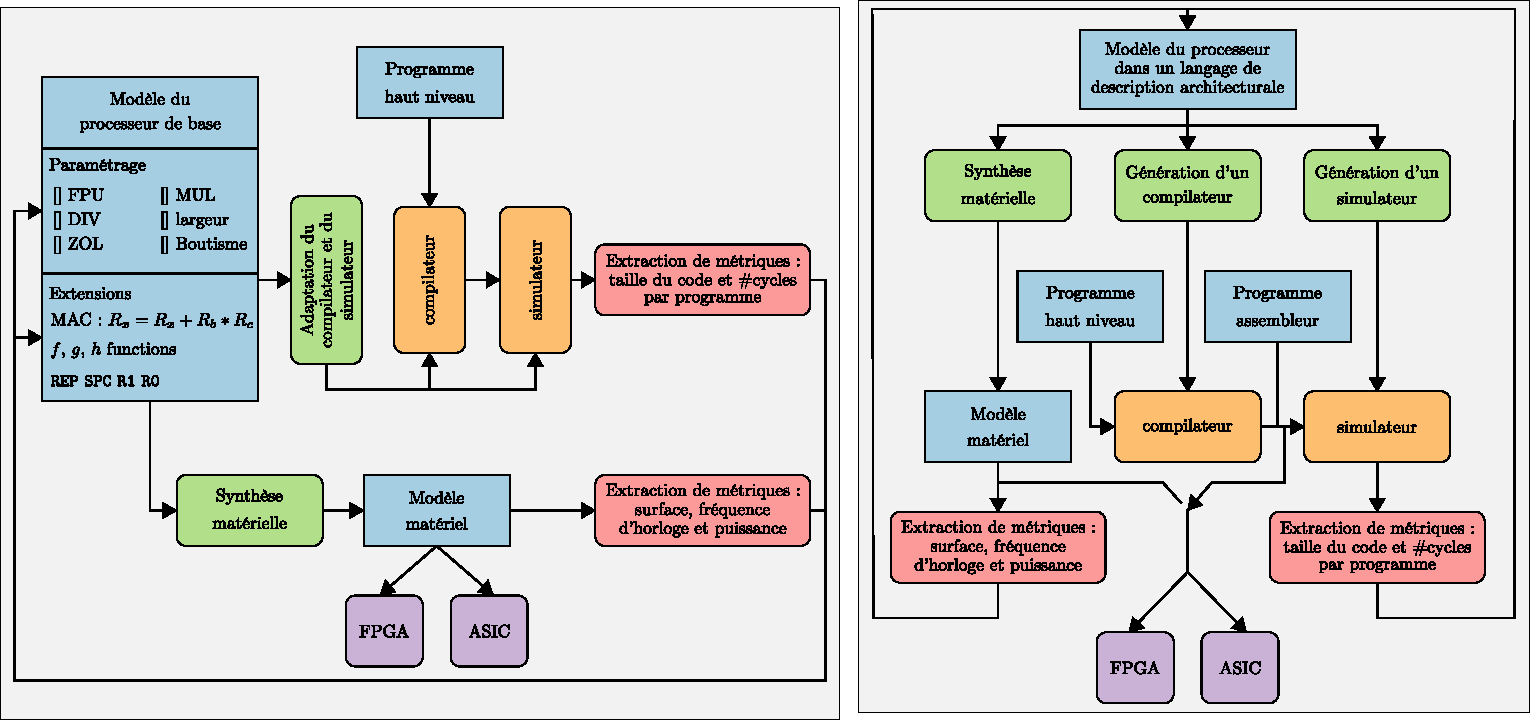
\includegraphics[width=0.9\textwidth]{./fig/methodos}
\end{frame}

\begin{frame}[c]{Approche Tensilica}
  \begin{columns}
    \begin{column}{.48\textwidth}
      \begin{itemize}
        \item Spécialisation d'un processeur de base
        \item Instructions spécialisées
        \item Environnement de développement complet
        \item<2-> Réduction de la consommation énergétique
      \end{itemize}
    \end{column}
    \begin{column}[T]{.48\textwidth}
    \only<+>
    {
      \vfill
      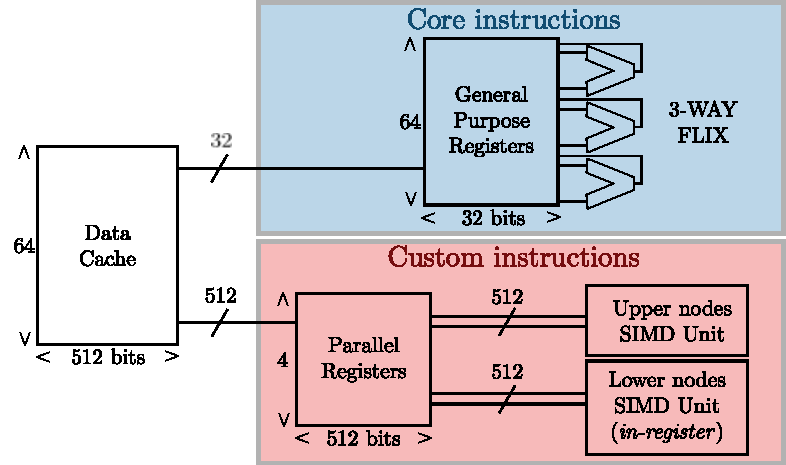
\includegraphics[width=\textwidth]{./fig/archi_tensilica}
      \vfill
    }
    \only<+->
    {
    \begin{table}[t]
      \centering
      {\small\resizebox{\linewidth}{!}{
      \begin{tabular}{c|c|c|c|c}
        \toprule

        Target & $N$ & \begin{tabular}{c}Latency\\{[$\mu$s]}\end{tabular} & \begin{tabular}{c}Throughput\\{[Mb/s]}\end{tabular} & \begin{tabular}{c}$E_b$\\{[nJ]}\end{tabular} \\

        \cmidrule(lr){1-1}
        \cmidrule(lr){2-2}
        \cmidrule(lr){3-5}
%                       
        \multirow{4}{*}{\bf A57-1.1GHz}  & $1024$   & $13$  & $38$  & \ORANGE{$21$} \\

                                         & $512$    & $6.7$ & $38$  & \ORANGE{$21$} \\

                                         & $256$    & $3.6$ & $35$  & \ORANGE{$22$}\\

                                         & $128$    & $2.1$ & $30$  & \ORANGE{$27$}\\

        \midrule

        \multirow{4}{*}{\bf i7-3.3GHz}   & $1024$   & $2.3$ & $222$ & \RED{$47$} \\

                                         & $512$    & $1.4$ & $182$ & \RED{$57$} \\

                                         & $256$    & $0.8$ & $155$ & \RED{$68$}\\

                                         & $128$    & $0.5$ & $124$ & \RED{$85$}\\

        \midrule

        \multirow{4}{*}{\bf ASIP-835MHz} & $1024$   & $7.2$ & $71$  & \GREEN{$1.6$} \\

                                         & $512$    & $3.9$ & $66$  & \GREEN{$1.7$} \\

                                         & $256$    & $1.9$ & $65$  & \GREEN{$1.7$}\\

                                         & $128$    & $1.0$ & $62$  & \GREEN{$1.8$}\\
        \bottomrule
      \end{tabular}
      }}
    \end{table}
    }
    \end{column}
  \end{columns}
\vfill
\centering
  \only<3>{Ce travail a fait l'objet d'une communication lors de la conférence ISCAS 2018.}
\end{frame}


\begin{frame}[c]{Limites de l'approche Tensilica}
  \begin{itemize}
    \item Langage de description matérielle spécifique
    \item Licence nécessaire
    \item Limitation de l'accès à la mémoire
    \item Rigidité de l'architecture
  \end{itemize}
\end{frame}

\begin{frame}[c]{Transport Triggered Architectures}
  \begin{itemize}
    \item Modèle de processeur
    \vspace{0.5cm}
    \item Similaire aux architectures VLIW
    \vspace{0.5cm}
    \item Parallélisme de données
    \vspace{0.5cm}
    \item Parallélisme d'instructions
  \end{itemize}
\end{frame}

\begin{frame}[c]{Structure d'un processeur TTA}
  \multiinclude[<+>][start=1,format=pdf,graphics={width=.8\textwidth}]{./fig/anim_tta_base}
\end{frame}

\begin{frame}[c]{Niveau de parallélisme}
  Two main polar functions : $f$ and $g$
  \vspace{1cm}

  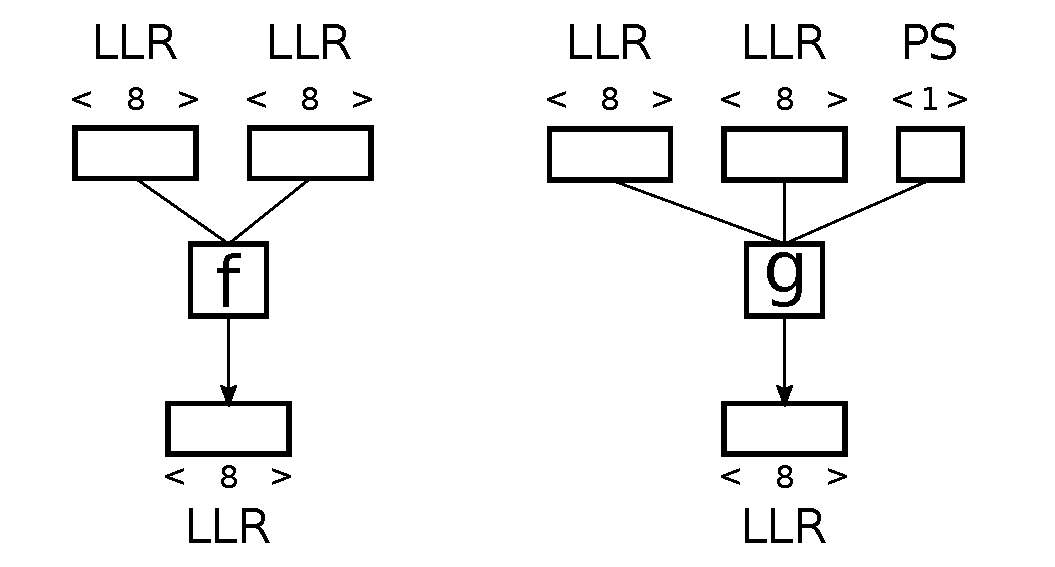
\includegraphics[width=0.7\textwidth]{fig/f_g_dimensions_scalar}
\end{frame}

\begin{frame}[c]{Niveau de parallélisme}
  Two main polar functions : $f$ and $g$
  \vspace{1cm}

  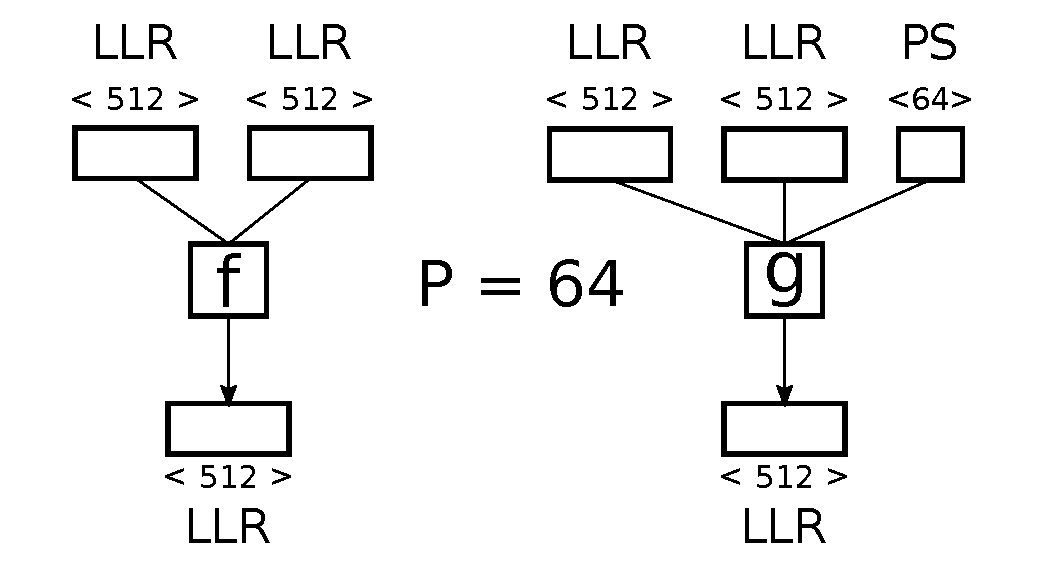
\includegraphics[width=0.7\textwidth]{fig/f_g_dimensions_vector}
\end{frame}

\begin{frame}[c]{Conception du processeur}
  \begin{columns}[T] % align columns
    \begin{column}{.48\textwidth}
      \vspace{-0.5cm}
      \multiinclude[<+>][start=1,format=pdf,graphics={width=1.4\textwidth}]{./fig/archi_sc_construction}
    \end{column}
    \begin{column}{.07\textwidth}
    \end{column}
    \begin{column}{.41\textwidth}
      \begin{itemize}
        \item<1-> Mémoires vectorielles
        \vspace{0.2cm}
        \item<2-> 2 bus de 512 bits
        \vspace{0.2cm}
        \item<2-> 1 bus de 64 bits
        \vspace{0.2cm}
        \item<3-> Unité de chargement et sauvegarde vectorielles
        \vspace{0.2cm}
        \item<4-> Unité de calcul polaire
      \end{itemize}
    \end{column}
  \end{columns} % align columns
\end{frame}

\begin{frame}[c]{Compilation}
  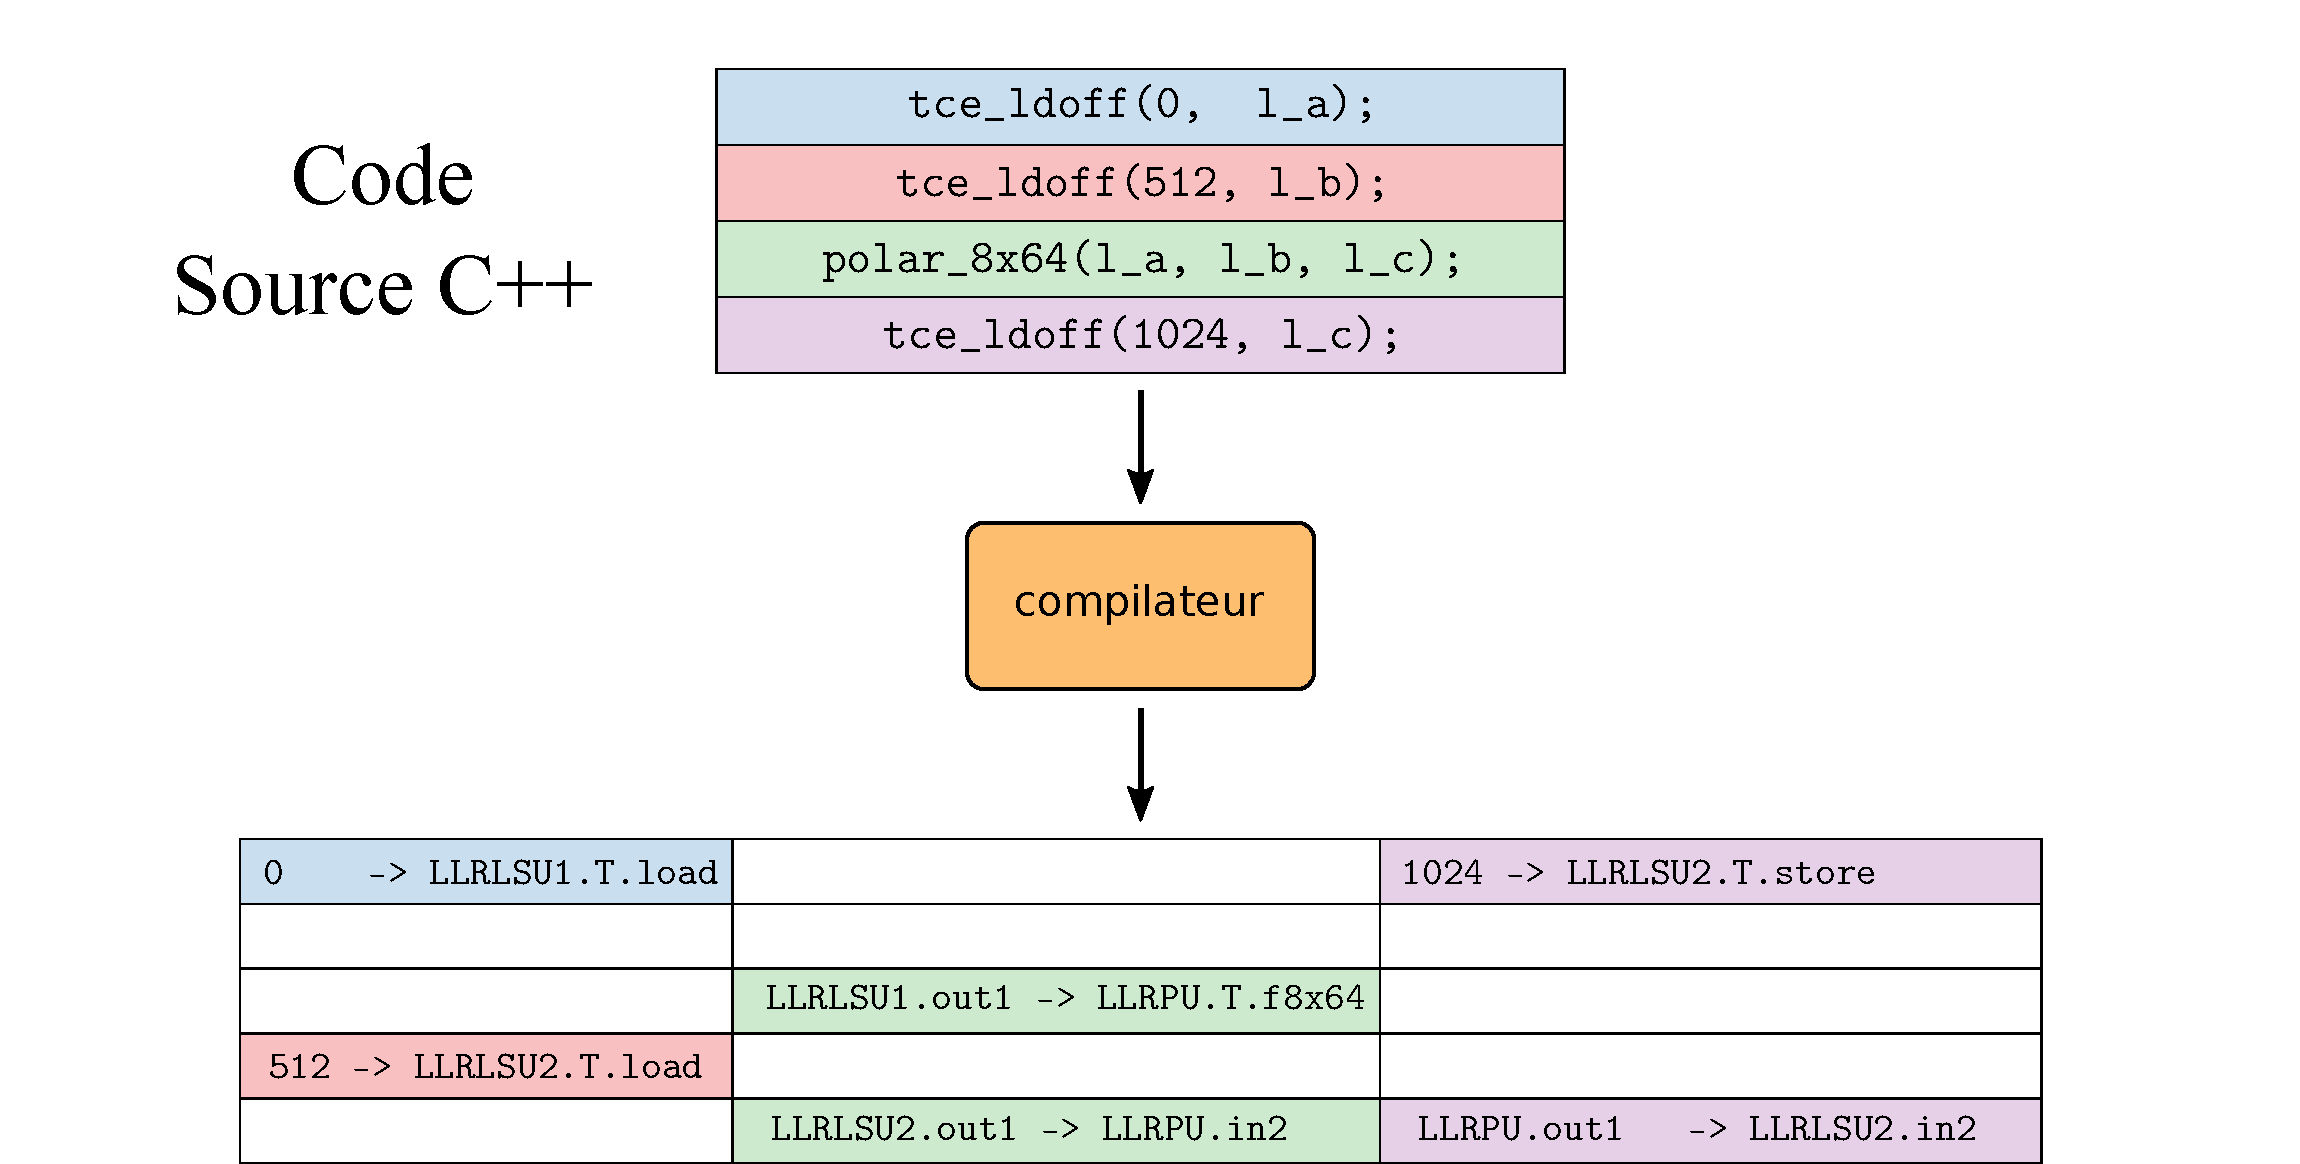
\includegraphics[width=\textwidth]{fig/compilation}
\end{frame}

\begin{frame}[c]{Parallélisme d'instruction}
  \multiinclude[<+>][start=1,format=pdf,graphics={width=.8\textwidth}]{./fig/ilp}
\end{frame}





\begin{frame}[c]{Comparaison avec des décodeurs logiciels}
  \begin{columns}[T] % align columns
  \begin{column}{.48\textwidth}
    \begin{itemize}
      \item<+-> Architecture proposée
      \item<+-> Processeurs Intel x86 (i7-4712HQ) et ARM (Cortex A57)
      \begin{itemize}
        \item<+-> Boîte à outils logicielle \textbf{AFF3CT}
        \item<+-> SIMD (Neon \& AVX2)
      \end{itemize}
      \item<+-> ASIP de type Tensilica
      \item<+-> Débit meximum atteint par le processeur proposé
      \item<+-> Consommation énergétique réduite d'un à deux ordres de grandeur
    \end{itemize}
  \end{column}

  \begin{column}{.48\textwidth}
  \only<1>{
    \begin{table}
      \centering
      {
      \small\resizebox{\linewidth}{!}{
      \begin{tabular}{c|c|c|c|c}
        \toprule

        Architecture & $N$ & \begin{tabular}{c}Latence\\{[$\mu$s]}\end{tabular} & \begin{tabular}{c}Débit\\{[Mb/s]}\end{tabular} & \begin{tabular}{c}$E_b$\\{[nJ/bit]}\end{tabular} \\

        \cmidrule(lr){1-1}
        \cmidrule(lr){2-2}
        \cmidrule(lr){3-5}

        \multirow{2}{*}{\bf \BLUE{TTPD-800MHz}}            & $1024$   & $1.4$  & $352$ & $0.14$ \\ % 1512 cycles
                                                    & $512$    & $0.8$  & $313$ & $0.15$ \\ % 803 cycles
        \multirow{2}{*}{\bf \BLUE{(ASIP)}}                 & $256$    & $0.4$  & $304$ & $0.16$ \\ % 413 cycles
                                                    & $128$    & $0.2$  & $284$ & $0.17$ \\ % 224 cycles
        \midrule
        \multirow{2}{*}{\bf i7-3.3GHz}              & $1024$   & $2.0$  & $257$ & $41$   \\
                                                    & $512$    & $1.2$  & $210$ & $49$   \\
        \multirow{2}{*}{\bf (GPP)}                  & $256$    & $0.7$  & $179$ & $59$   \\
                                                    & $128$    & $0.4$  & $143$ & $73$   \\
        \midrule    
        \multirow{2}{*}{\bf A57-1.1GHz}             & $1024$   & $10.7$ & $48$  & $17$   \\
                                                    & $512$    & $5.3$  & $48$  & $17$   \\
        \multirow{2}{*}{\bf (GPP)}                  & $256$    & $2.8$  & $46$  & $17$   \\
                                                    & $128$    & $1.6$  & $41$  & $20$   \\
        \midrule
        \multirow{2}{*}{\bf LX7-835MHz}             & $1024$   & $7.2$  & $71$  & $1.6$  \\
                                                    & $512$    & $3.9$  & $66$  & $1.7$  \\
        \multirow{2}{*}{\bf (ASIP)}                 & $256$    & $1.9$  & $65$  & $1.7$  \\
                                                    & $128$    & $1.0$  & $62$  & $1.8$  \\
        \bottomrule
      \end{tabular}
      }}
    \end{table}
  }
    
    \only<2-4>{
    \begin{table}
      \centering
      {
      \small\resizebox{\linewidth}{!}{
      \begin{tabular}{c|c|c|c|c}
        \toprule

        Architecture & $N$ & \begin{tabular}{c}Latence\\{[$\mu$s]}\end{tabular} & \begin{tabular}{c}Débit\\{[Mb/s]}\end{tabular} & \begin{tabular}{c}$E_b$\\{[nJ/bit]}\end{tabular} \\

        \cmidrule(lr){1-1}
        \cmidrule(lr){2-2}
        \cmidrule(lr){3-5}


        \multirow{2}{*}{\bf TTPD-800MHz}            & $1024$   & $1.4$  & $352$ & $0.14$ \\ % 1512 cycles
                                                    & $512$    & $0.8$  & $313$ & $0.15$ \\ % 803 cycles
        \multirow{2}{*}{\bf (ASIP)}                 & $256$    & $0.4$  & $304$ & $0.16$ \\ % 413 cycles
                                                    & $128$    & $0.2$  & $284$ & $0.17$ \\ % 224 cycles
        \midrule
        \multirow{2}{*}{\bf \BLUE{i7-3.3GHz}}       & $1024$   & $2.0$  & $257$ & $41$   \\
                                                    & $512$    & $1.2$  & $210$ & $49$   \\
        \multirow{2}{*}{\bf \BLUE{(GPP)}}           & $256$    & $0.7$  & $179$ & $59$   \\
                                                    & $128$    & $0.4$  & $143$ & $73$   \\
        \midrule    
        \multirow{2}{*}{\bf \BLUE{A57-1.1GHz}}      & $1024$   & $10.7$ & $48$  & $17$   \\
                                                    & $512$    & $5.3$  & $48$  & $17$   \\
        \multirow{2}{*}{\bf \BLUE{(GPP)}}           & $256$    & $2.8$  & $46$  & $17$   \\
                                                    & $128$    & $1.6$  & $41$  & $20$   \\
        \midrule
        \multirow{2}{*}{\bf LX7-835MHz}             & $1024$   & $7.2$  & $71$  & $1.6$  \\
                                                    & $512$    & $3.9$  & $66$  & $1.7$  \\
        \multirow{2}{*}{\bf (ASIP)}                 & $256$    & $1.9$  & $65$  & $1.7$  \\
                                                    & $128$    & $1.0$  & $62$  & $1.8$  \\
        \bottomrule
      \end{tabular}
      }}
    \end{table}
    }

  \only<5>{
    \begin{table}
      \centering
      {
      \small\resizebox{\linewidth}{!}{
      \begin{tabular}{c|c|c|c|c}
        \toprule

        Architecture & $N$ & \begin{tabular}{c}Latence\\{[$\mu$s]}\end{tabular} & \begin{tabular}{c}Débit\\{[Mb/s]}\end{tabular} & \begin{tabular}{c}$E_b$\\{[nJ/bit]}\end{tabular} \\

        \cmidrule(lr){1-1}
        \cmidrule(lr){2-2}
        \cmidrule(lr){3-5}


        \multirow{2}{*}{\bf TTPD-800MHz}            & $1024$   & $1.4$  & $352$ & $0.14$ \\ % 1512 cycles
                                                    & $512$    & $0.8$  & $313$ & $0.15$ \\ % 803 cycles
        \multirow{2}{*}{\bf (ASIP)}                 & $256$    & $0.4$  & $304$ & $0.16$ \\ % 413 cycles
                                                    & $128$    & $0.2$  & $284$ & $0.17$ \\ % 224 cycles
        \midrule
        \multirow{2}{*}{\bf i7-3.3GHz}              & $1024$   & $2.0$  & $257$ & $41$   \\
                                                    & $512$    & $1.2$  & $210$ & $49$   \\
        \multirow{2}{*}{\bf (GPP)}                  & $256$    & $0.7$  & $179$ & $59$   \\
                                                    & $128$    & $0.4$  & $143$ & $73$   \\
        \midrule    
        \multirow{2}{*}{\bf A57-1.1GHz}             & $1024$   & $10.7$ & $48$  & $17$   \\
                                                    & $512$    & $5.3$  & $48$  & $17$   \\
        \multirow{2}{*}{\bf (GPP)}                  & $256$    & $2.8$  & $46$  & $17$   \\
                                                    & $128$    & $1.6$  & $41$  & $20$   \\
        \midrule
        \multirow{2}{*}{\bf \BLUE{LX7-835MHz}}      & $1024$   & $7.2$  & $71$  & $1.6$  \\
                                                    & $512$    & $3.9$  & $66$  & $1.7$  \\
        \multirow{2}{*}{\bf \BLUE{(ASIP)}}          & $256$    & $1.9$  & $65$  & $1.7$  \\
                                                    & $128$    & $1.0$  & $62$  & $1.8$  \\

        \bottomrule
      \end{tabular}
      }}
    \end{table}
    }
    \only<6>{
    \begin{table}
      \centering
      {
      \small\resizebox{\linewidth}{!}{
      \begin{tabular}{c|c|c|c|c}
        \toprule

        Architecture & $N$ & \begin{tabular}{c}Latence\\{[$\mu$s]}\end{tabular} & \begin{tabular}{c}Débit\\{[Mb/s]}\end{tabular} & \begin{tabular}{c}$E_b$\\{[nJ/bit]}\end{tabular} \\

        \cmidrule(lr){1-1}
        \cmidrule(lr){2-2}
        \cmidrule(lr){3-5}


        \multirow{2}{*}{\bf TTPD-800MHz}            & $1024$   & $1.4$  & \GREEN{$\mathbf{352}$} & $0.14$ \\ % 1512 cycles
                                                    & $512$    & $0.8$  & \GREEN{$\mathbf{313}$} & $0.15$ \\ % 803 cycles
        \multirow{2}{*}{\bf (ASIP)}                 & $256$    & $0.4$  & \GREEN{$\mathbf{304}$} & $0.16$ \\ % 413 cycles
                                                    & $128$    & $0.2$  & \GREEN{$\mathbf{284}$} & $0.17$ \\ % 224 cycles
        \midrule
        \multirow{2}{*}{\bf i7-3.3GHz}              & $1024$   & $2.0$  & \GREEN{$\mathbf{257}$} & $41$   \\
                                                    & $512$    & $1.2$  & \GREEN{$\mathbf{210}$} & $49$   \\
        \multirow{2}{*}{\bf (GPP)}                  & $256$    & $0.7$  & \GREEN{$\mathbf{179}$} & $59$   \\
                                                    & $128$    & $0.4$  & \GREEN{$\mathbf{143}$} & $73$   \\
        \midrule    
        \multirow{2}{*}{\bf A57-1.1GHz}             & $1024$   & $10.7$ & \ORANGE{$\mathbf{48}$} & $17$   \\
                                                    & $512$    & $5.3$  & \ORANGE{$\mathbf{48}$} & $17$   \\
        \multirow{2}{*}{\bf (GPP)}                  & $256$    & $2.8$  & \ORANGE{$\mathbf{46}$} & $17$   \\
                                                    & $128$    & $1.6$  & \ORANGE{$\mathbf{41}$} & $20$   \\
        \midrule
        \multirow{2}{*}{\bf LX7-835MHz}             & $1024$   & $7.2$  & \ORANGE{$\mathbf{71}$} & $1.6$  \\
                                                    & $512$    & $3.9$  & \ORANGE{$\mathbf{66}$} & $1.7$  \\
        \multirow{2}{*}{\bf (ASIP)}                 & $256$    & $1.9$  & \ORANGE{$\mathbf{65}$} & $1.7$  \\
                                                    & $128$    & $1.0$  & \ORANGE{$\mathbf{62}$} & $1.8$  \\

        \bottomrule
      \end{tabular}
      }}
    \end{table}
    }
    \only<7>{
    \begin{table}
      \centering
      {
      \small\resizebox{\linewidth}{!}{
      \begin{tabular}{c|c|c|c|c}
        \toprule

        Architecture & $N$ & \begin{tabular}{c}Latence\\{[$\mu$s]}\end{tabular} & \begin{tabular}{c}Débit\\{[Mb/s]}\end{tabular} & \begin{tabular}{c}$E_b$\\{[nJ/bit]}\end{tabular} \\

        \cmidrule(lr){1-1}
        \cmidrule(lr){2-2}
        \cmidrule(lr){3-5}


        \multirow{2}{*}{\bf TTPD-800MHz}            & $1024$   & $1.4$  & $352$ & \GREEN{$\mathbf{0.14}$} \\ % 1512 cycles
                                                    & $512$    & $0.8$  & $313$ & \GREEN{$\mathbf{0.15}$} \\ % 803 cycles
        \multirow{2}{*}{\bf (ASIP)}                 & $256$    & $0.4$  & $304$ & \GREEN{$\mathbf{0.16}$} \\ % 413 cycles
                                                    & $128$    & $0.2$  & $284$ & \GREEN{$\mathbf{0.17}$} \\ % 224 cycles
        \midrule
        \multirow{2}{*}{\bf i7-3.3GHz}              & $1024$   & $2.0$  & $257$ & \RED{$\mathbf{41}$}   \\
                                                    & $512$    & $1.2$  & $210$ & \RED{$\mathbf{49}$}   \\
        \multirow{2}{*}{\bf (GPP)}                  & $256$    & $0.7$  & $179$ & \RED{$\mathbf{59}$}   \\
                                                    & $128$    & $0.4$  & $143$ & \RED{$\mathbf{73}$}   \\
        \midrule    
        \multirow{2}{*}{\bf A57-1.1GHz}             & $1024$   & $10.7$ & $48$  & \RED{$\mathbf{17}$}   \\
                                                    & $512$    & $5.3$  & $48$  & \RED{$\mathbf{17}$}   \\
        \multirow{2}{*}{\bf (GPP)}                  & $256$    & $2.8$  & $46$  & \RED{$\mathbf{17}$}   \\
                                                    & $128$    & $1.6$  & $41$  & \RED{$\mathbf{20}$}   \\
        \midrule
        \multirow{2}{*}{\bf LX7-835MHz}             & $1024$   & $7.2$  & $71$  & \ORANGE{$\mathbf{1.6}$}  \\
                                                    & $512$    & $3.9$  & $66$  & \ORANGE{$\mathbf{1.7}$}  \\
        \multirow{2}{*}{\bf (ASIP)}                 & $256$    & $1.9$  & $65$  & \ORANGE{$\mathbf{1.7}$}  \\
                                                    & $128$    & $1.0$  & $62$  & \ORANGE{$\mathbf{1.8}$}  \\

        \bottomrule
      \end{tabular}
      }}
    \end{table}
    }
  \end{column}
  \end{columns}
\end{frame}


\begin{frame}[c]{Comparaison avec des architectures matérielles dédiées}
    \begin{itemize}
      \item<+-> Processeur proposé
      \item<+-> Décodeur matériel dédié
      \item<2-> Décodeur matériel dédié avec construction optimisée
      \item<+-> Implémentations FPGA
    \end{itemize}

    \only<1>{
      \begin{table}
      \centering
      {
        \small\resizebox{0.8\linewidth}{!}{
        \begin{tabular}{c|c|c|c|c}
                                  & \BLUE{TTPD Proposé}  & \cite{giard_638_2015} & \multicolumn{2}{c}{\cite{sarkis2014fast}} \\
          \cmidrule(lr){2-2}
          \cmidrule(lr){3-3}
          \cmidrule(lr){4-5}

          \textbf{FPGA}               &  Artix 7       & Stratix IV            & Stratix IV         & Virtex 6             \\
          \textbf{Cycles d'horloge}   &  1161          & 222                   & 165                & 165                  \\
          \textbf{\'Elagage}          &  R0 \& R1      & Complet               & Complet            & Complet              \\
          \textbf{LUTS}               &  14744         & 23020                 & 24821              & 22115                \\
          \textbf{RAM} (Kb)           &  141           & 43                    & 36                 & 36                   \\

        \end{tabular}
      }}
      \end{table}
    }

    \only<2>{
      \begin{table}
      \centering
      {
        \small\resizebox{0.8\linewidth}{!}{
        \begin{tabular}{c|c|c|c|c}
                                  & TTPD Proposé  & \BLUE{\cite{giard_638_2015}} & \multicolumn{2}{c}{\BLUE{\cite{sarkis2014fast}}} \\
          \cmidrule(lr){2-2}
          \cmidrule(lr){3-3}
          \cmidrule(lr){4-5}

          \textbf{FPGA}         &  Artix 7       & Stratix IV            & Stratix IV         & Virtex 6             \\
          \textbf{Cycles d'horloge}   &  1161          & 222                   & 165                & 165                  \\
          \textbf{\'Elagage}        &  R0 \& R1      & Complet                  & Complet               & Complet                 \\
          \textbf{LUTS}           &  14744         & 23020                 & 24821              & 22115                \\
          \textbf{RAM} (Kb)       &  141           & 43                    & 36                 & 36                   \\

        \end{tabular}
      }}
      \end{table}
    }

    \only<3>{
      \begin{table}
      \centering
      {
        \small\resizebox{0.8\linewidth}{!}{
        \begin{tabular}{c|c|c|c|c}
                                  & TTPD Proposé  & \cite{giard_638_2015} & \multicolumn{2}{c}{\cite{sarkis2014fast}} \\
          \cmidrule(lr){2-2}
          \cmidrule(lr){3-3}
          \cmidrule(lr){4-5}

          \textbf{FPGA}         &  \textbf{Artix 7}       & \textbf{Stratix IV}            & \textbf{Stratix IV }        & \textbf{Virtex 6}             \\
          \textbf{Cycles d'horloge}   &  1161          & 222                   & 165                & 165                  \\
          \textbf{\'Elagage}        &  R0 \& R1      & Complet                  & Complet               & Complet                 \\
          \textbf{LUTS}           &  14744         & 23020                 & 24821              & 22115                \\
          \textbf{RAM} (Kb)       &  141           & 43                    & 36                 & 36                   \\

        \end{tabular}
      }}
      \end{table}
    }
\end{frame}

\begin{frame}[c]{Comparaison avec des architectures matérielles dédiées}
    \begin{itemize}
      \item<+-> 5 à six fois plus de cycles
      \item<+-> Différents niveaux d'élagage
      \item<+-> Plus petit nombre de LUTs
      \item<+-> Plus grosse empreinte mémoire
    \end{itemize}

    \only<1>{
      \begin{table}
      \centering
      {
        \small\resizebox{0.8\linewidth}{!}{
        \begin{tabular}{c|c|c|c|c}
                                  & TTPD Proposé  & \cite{giard_638_2015} & \multicolumn{2}{c}{\cite{sarkis2014fast}} \\
          \cmidrule(lr){2-2}
          \cmidrule(lr){3-3}
          \cmidrule(lr){4-5}

          \textbf{FPGA}         &  Artix 7       & Stratix IV            & Stratix IV         & Virtex 6             \\
          \textbf{Cycles d'horloge}   &  \textbf{1161}  & \textbf{222}           & \textbf{165}        & \textbf{165}          \\
          \textbf{\'Elagage}        &  R0 \& R1      & Complet                  & Complet               & Complet                 \\
          \textbf{LUTS}           &  14744         & 23020                 & 24821              & 22115                \\
          \textbf{RAM} (Kb)       &  141           & 43                    & 36                 & 36                   \\

        \end{tabular}
      }}
      \end{table}
    }
    \only<2>{
      \begin{table}
      \centering
      {
        \small\resizebox{0.8\linewidth}{!}{
        \begin{tabular}{c|c|c|c|c}
                                  & TTPD Proposé  & \cite{giard_638_2015} & \multicolumn{2}{c}{\cite{sarkis2014fast}} \\
          \cmidrule(lr){2-2}
          \cmidrule(lr){3-3}
          \cmidrule(lr){4-5}

          \textbf{FPGA}         &  Artix 7       & Stratix IV            & Stratix IV         & Virtex 6             \\
          \textbf{Cycles d'horloge}   &  1161          & 222                   & 165                & 165                  \\
          \textbf{\'Elagage}        &  \textbf{R0 \& R1}      & \textbf{Complet}                  & \textbf{Complet}               & \textbf{Complet}                 \\
          \textbf{LUTS}           &  14744         & 23020                 & 24821              & 22115                \\
          \textbf{RAM} (Kb)       &  141           & 43                    & 36                 & 36                   \\

        \end{tabular}
      }}
      \end{table}
    }
    \only<3>{
      \begin{table}
      \centering
      {
        \small\resizebox{0.8\linewidth}{!}{
        \begin{tabular}{c|c|c|c|c}
                                  & TTPD Proposé  & \cite{giard_638_2015} & \multicolumn{2}{c}{\cite{sarkis2014fast}} \\
          \cmidrule(lr){2-2}
          \cmidrule(lr){3-3}
          \cmidrule(lr){4-5}

          \textbf{FPGA}         &  Artix 7        & Stratix IV             & Stratix IV          & Virtex 6              \\
          \textbf{Cycles d'horloge}   &  1161           & 222                    & 165                 & 165                   \\
          \textbf{\'Elagage}        &  R0 \& R1       & Complet                   & Complet                & Complet                  \\
          \textbf{LUTS}           &  \textbf{14744} & \textbf{23020}         & \textbf{24821}      & \textbf{22115}        \\
          \textbf{RAM} (Kb)       &  141            & 43                     & 36                  & 36                    \\


        \end{tabular}
      }}
      \end{table}
    }
    \only<4>{
      \begin{table}
      \centering
      {
        \small\resizebox{0.8\linewidth}{!}{
        \begin{tabular}{c|c|c|c|c}
                                  & TTPD Proposé  & \cite{giard_638_2015} & \multicolumn{2}{c}{\cite{sarkis2014fast}} \\
          \cmidrule(lr){2-2}
          \cmidrule(lr){3-3}
          \cmidrule(lr){4-5}

          \textbf{FPGA}         &  Artix 7       & Stratix IV            & Stratix IV         & Virtex 6             \\
          \textbf{Cycles d'horloge}   &  1161          & 222                   & 165                & 165                  \\
          \textbf{\'Elagage}        &  R0 \& R1      & Complet                  & Complet               & Complet                  \\
          \textbf{LUTS}           &  14744         & 23020                 & 24821              & 22115                \\
          \textbf{RAM} (Kb)       &  \textbf{141}  & \textbf{43}           & \textbf{36}        & \textbf{36}          \\


        \end{tabular}
      }}
      \end{table}
    }
\end{frame}

\section{Conclusion et perspectives}
\subsection*{}

\begin{frame}[c]{Conclusion}

  \begin{itemize}
    \item<+-> Premier décodeur polaire TTA
    \vspace{0.3cm}
    \item<+-> Meilleure efficacité énergétique que pour des processeurs embarqués
    \vspace{0.3cm}
    \item<+-> Architecture modulaire et adaptive (implémentation de l'algorithme SCAN)
    \vspace{0.3cm}
    \item<+-> Perspectives
    \begin{itemize}
      \item<+-> Algorithme SCL
      \item<+-> Multicœur
    \end{itemize}
  \end{itemize}

\end{frame}

\begin{frame}[allowframebreaks]{References}
\printbibliography
\end{frame}
